% !Mode:: "TeX:UTF-8"
\documentclass{article}
\usepackage[hyperref, UTF8]{ctex}
\usepackage[dvipsnames]{xcolor}
\usepackage{geometry}
\usepackage{amsmath}
\usepackage{amsfonts}
\usepackage{listings}
\usepackage{pgfplotstable}
\usepackage{pgfplots}
\usepackage{fontspec}
\usepackage{booktabs} % 表格上的不同横线
%\setmainfont{Consolas} %设置英文字体

\definecolor{mygreen}{rgb}{0,0.6,0}
\definecolor{mygray}{rgb}{0.5,0.5,0.5}
\definecolor{mymauve}{rgb}{0.58,0,0.82}
\lstset{ %
    backgroundcolor=\color{white},   % choose the background color
    basicstyle=\footnotesize\ttfamily,        % size of fonts used for the code
    columns=fullflexible,
    breaklines=true,                 % automatic line breaking only at whitespace
    captionpos=b,                    % sets the caption-position to bottom
    tabsize=4,
    backgroundcolor=\color[RGB]{245,245,244},            % 设定背景颜色
    commentstyle=\color{mygreen},    % comment style
    escapeinside={\%*}{*)},          % if you want to add LaTeX within your code
    keywordstyle=\color{blue},       % keyword style
    stringstyle=\color{mymauve}\ttfamily,     % string literal style
    showstringspaces=false,                % 不显示字符串中的空格
    frame=none,
    rulesepcolor=\color{red!20!green!20!blue!20},
    % identifierstyle=\color{red},
    language=c++,
}

% 设置hyperlink的颜色
\newcommand\myshade{85}
\colorlet{mylinkcolor}{violet}
\colorlet{mycitecolor}{YellowOrange}
\colorlet{myurlcolor}{Aquamarine}


\title{软件测试报告}
\author{Tomato}
\date{2018年1月}

\begin{document}

	\maketitle
		\section{引言}
			\subsection{文档概述}
				本文档将介绍测试的详细结果,主要是Coverage。
		\section{测试结果概述}
			\subsection{对被测试软件的总体评估}
				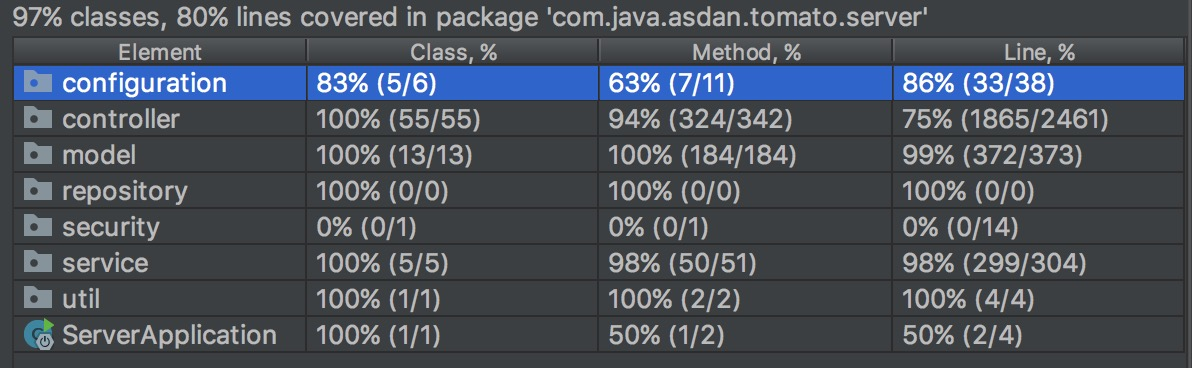
\includegraphics[scale = .3]{fig/test_1.jpg}

				本测试覆盖率很高,可以说是十分到位了。
			\subsection{测试环境的影响}
				任何平台都可以进行测试,并没有什么影响。
			\subsection{改进建议}
				如果可以的话,可以绕出架构对微信的websocket进行测试。
		\section{详细的测试结果}
			以下是我们的测试覆盖率:

			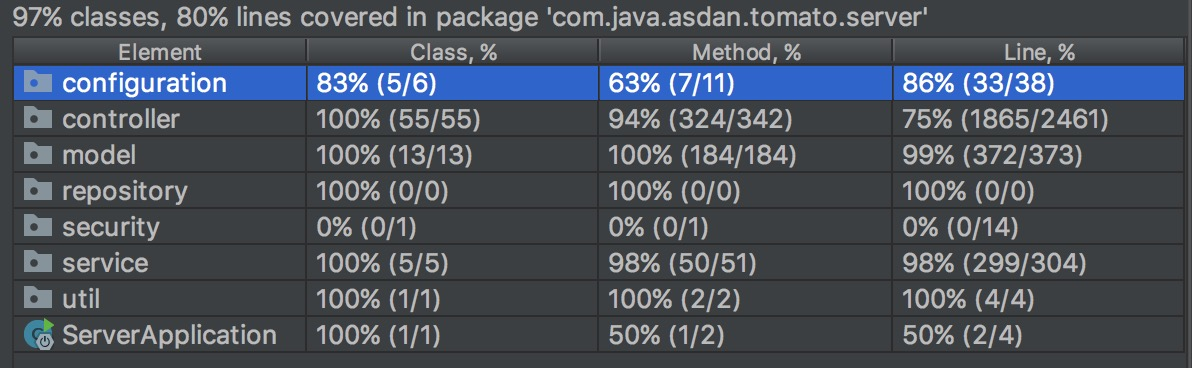
\includegraphics[scale = .3]{fig/test_1.jpg}
		
			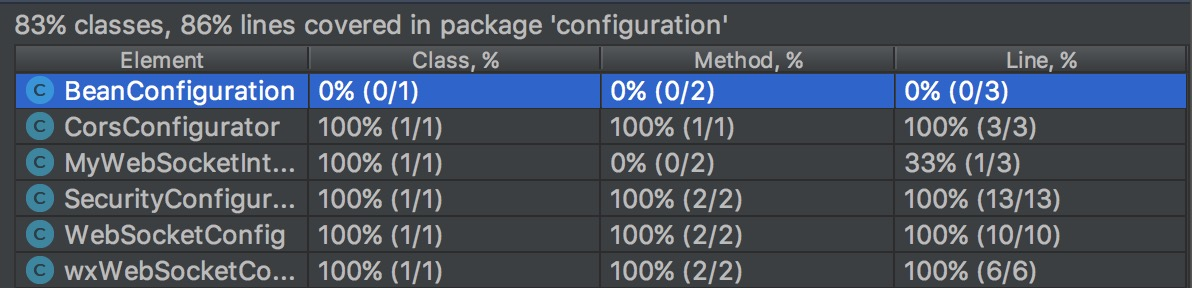
\includegraphics[scale = .3]{fig/test_2.jpg}
		
			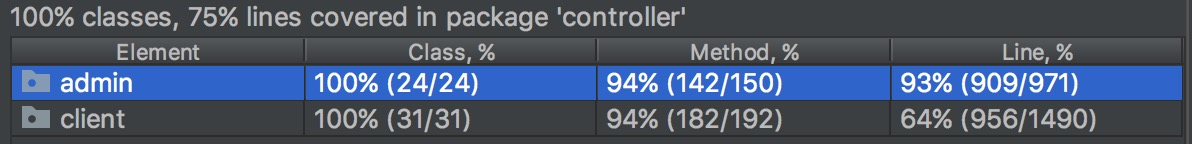
\includegraphics[scale = .3]{fig/test_3.jpg}
		
			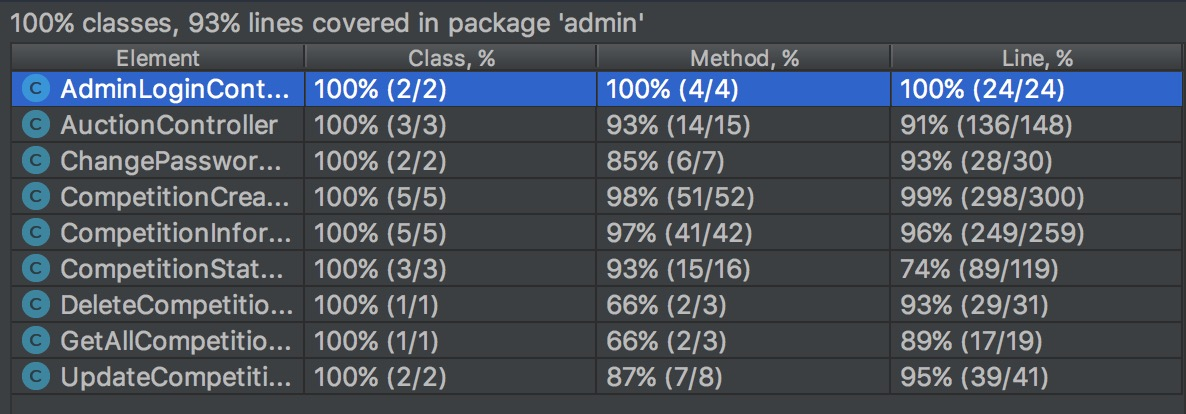
\includegraphics[scale = .3]{fig/test_4.jpg}
		
			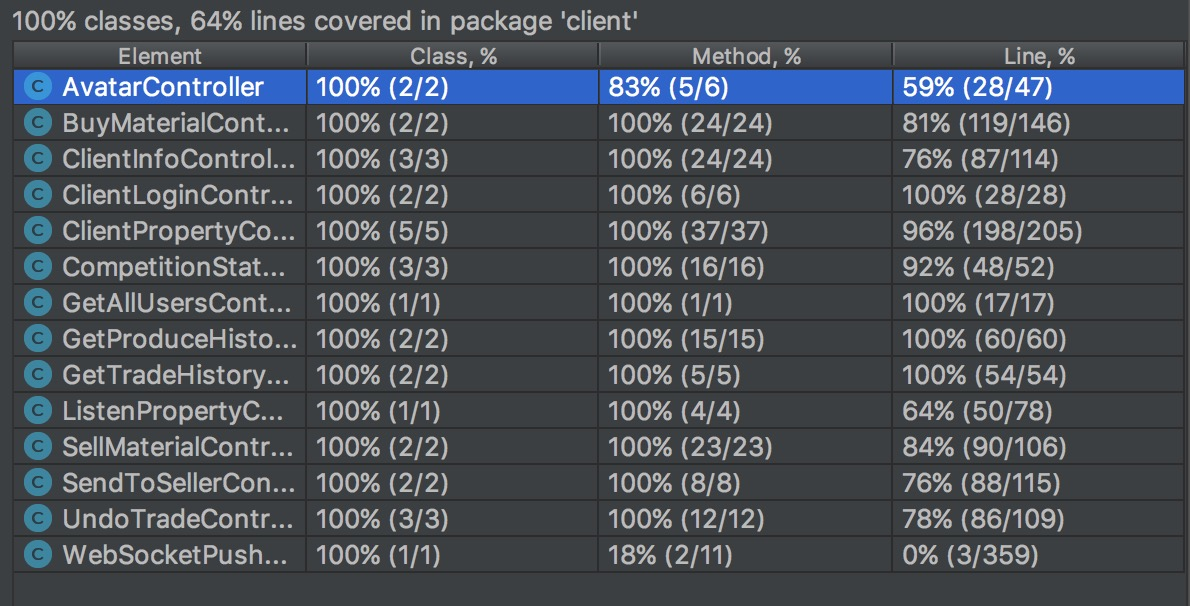
\includegraphics[scale = .3]{fig/test_5.jpg}
		
			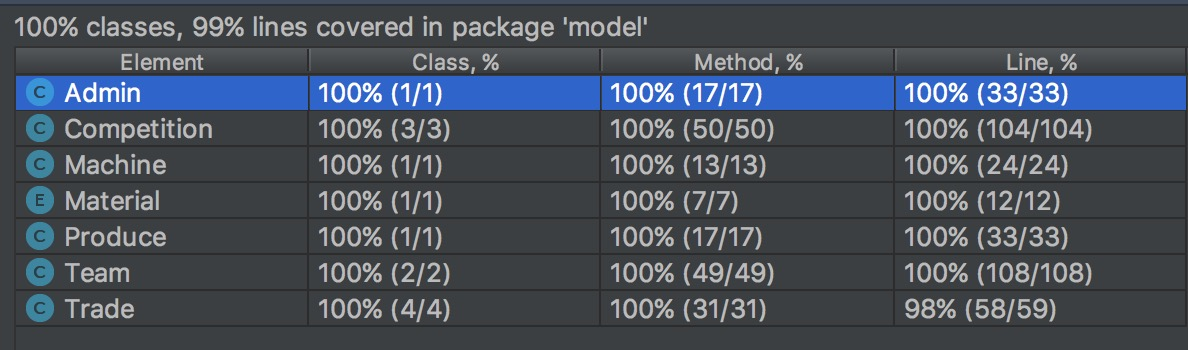
\includegraphics[scale = .3]{fig/test_6.jpg}
		
			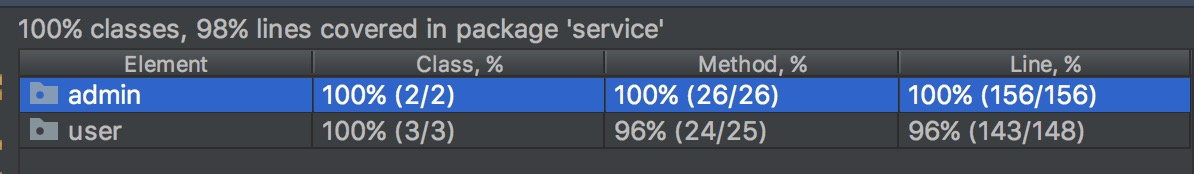
\includegraphics[scale = .3]{fig/test_7.jpg}
		
			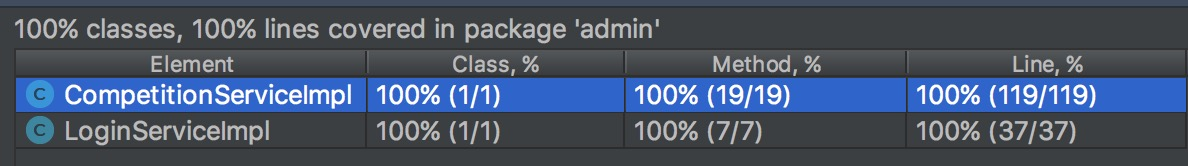
\includegraphics[scale = .3]{fig/test_8.jpg}
		
			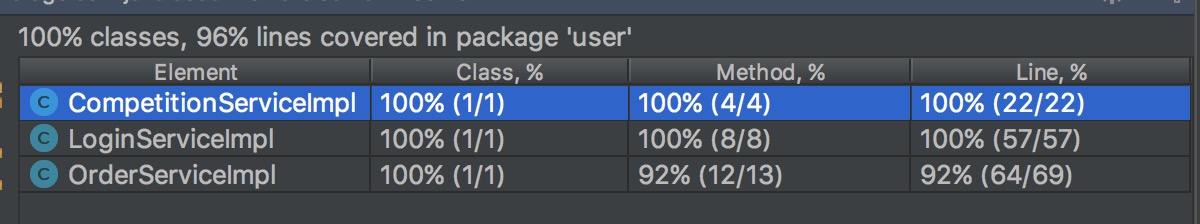
\includegraphics[scale = .3]{fig/test_9.jpg}
		\section{测试记录}
			本次测试结果生成于2018年1月19日,测试平台是Mac,集成开发环境是IntelliJ。见证者是宋世虹和张慧盟。
		\section{评价}
			\subsection{能力}
				该测试覆盖了几乎所有后台的接口,可以说是很鲁棒,给前端提供了十分稳定的服务。
			\subsection{缺陷和限制}
				由于没有找到微信的websocket的测试方法,所以我们没有对微信的websocket进行测试,这很遗憾。同时,由于时间的关系,还有极少一部分代码没有被测试到。
		\section{测试活动总结}
			人力消耗:张慧盟、宋世虹。


\end{document}
